\section{Модальное управление}
Рассмотрим модальный регулятор вида $u = Kx$. Согласно (\ref{eq:controlability_matrix}), система является 
полностью управляемой. Таким образом, любой спектр замкнутой системы является достижимым. 
Выберем желаемый спектр для замкнутой регулятор системы $\sigma_1 = \begin{bmatrix}-3 & -3 & -2 & -2\end{bmatrix}$. 
Для реализации регулятора, обеспечивающего заданный спектр, воспользуемся уравнением Сильвестра: 
\begin{equation}
    \begin{cases}
        AP - P\Gamma = BY \\
        K = -YP^{-1} 
    \end{cases}
\end{equation}
где $\Gamma$ -- матрица с желаемым спектром. 
Решение данного уравнения существует, при условии того, что пара $(Y, \Gamma)$ является наблюдаемой.

Решим данное уравнение с помощью пакета \texttt{cvx} в MATLAB, в результате получаем матрицу регулятора $K$:
\begin{equation}
     K = \begin{bmatrix}
    -11035.11  & -22635.99  & -6541.54  & -1534.51 \\ 
    \end{bmatrix}
\end{equation} 

Проверим правильность полученного результата, вычислив собственные числа замкнутой системы $A + BK$: 
\begin{equation}
    \sigma(A + BK) = \begin{bmatrix}
    -3.00 \\ 
    -3.00 \\ 
    -2.00 \\ 
    -2.00 \\ 
    \end{bmatrix}
\end{equation}
Получены желаемые собственные числа, что подтверждает правильность полученного результата. 
Рассмотрим работу регулятора на линейной модели системы при отсутствии внешних возмущений и 
небольшом начальном отклонении от равновесного состояния ($\theta_0 = 0.2$). Схема моделирования приведена на 
рисунке \ref{fig:modal_control_scheme_linear}. Результаты моделирования приведены на 
рисунке \ref{fig:modal_control_linear_out}.

\begin{figure}[ht!]
    \centering
    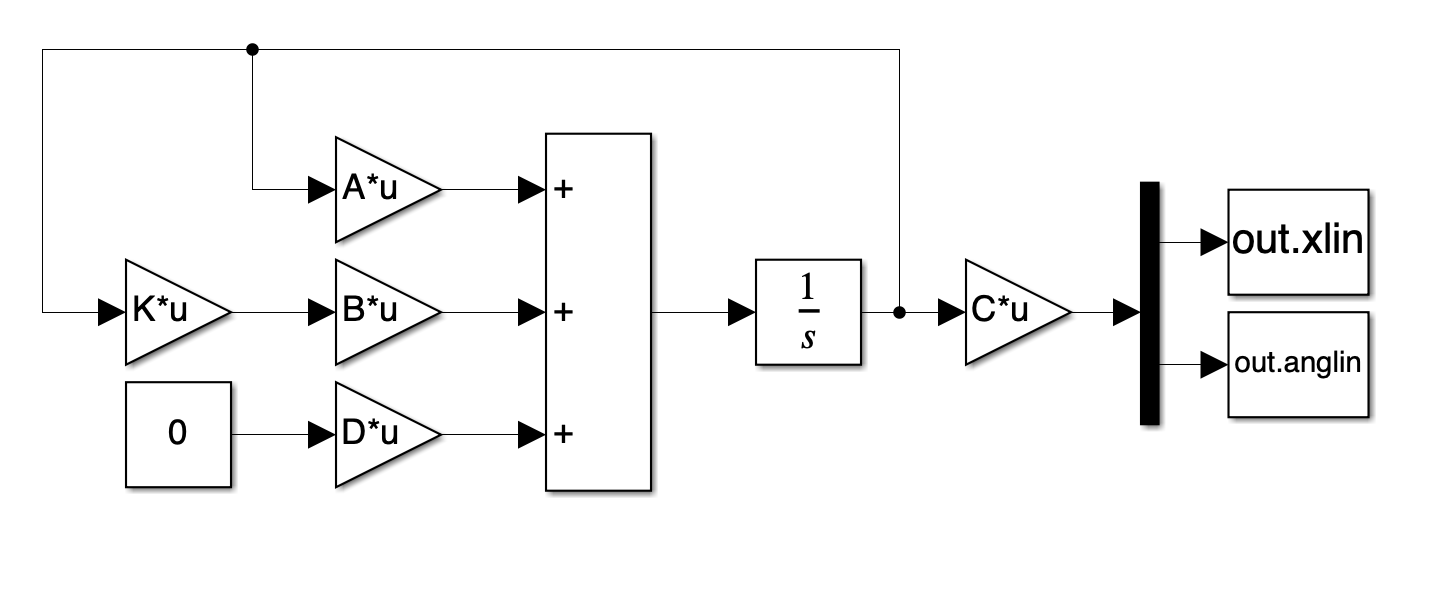
\includegraphics[width=\textwidth]{media/modal_control_linear.png}
    \caption{Схема моделирования линейной модели системы с модальным регулятором}
    \label{fig:modal_control_scheme_linear}
\end{figure}
\begin{figure}[ht!]
    \centering
    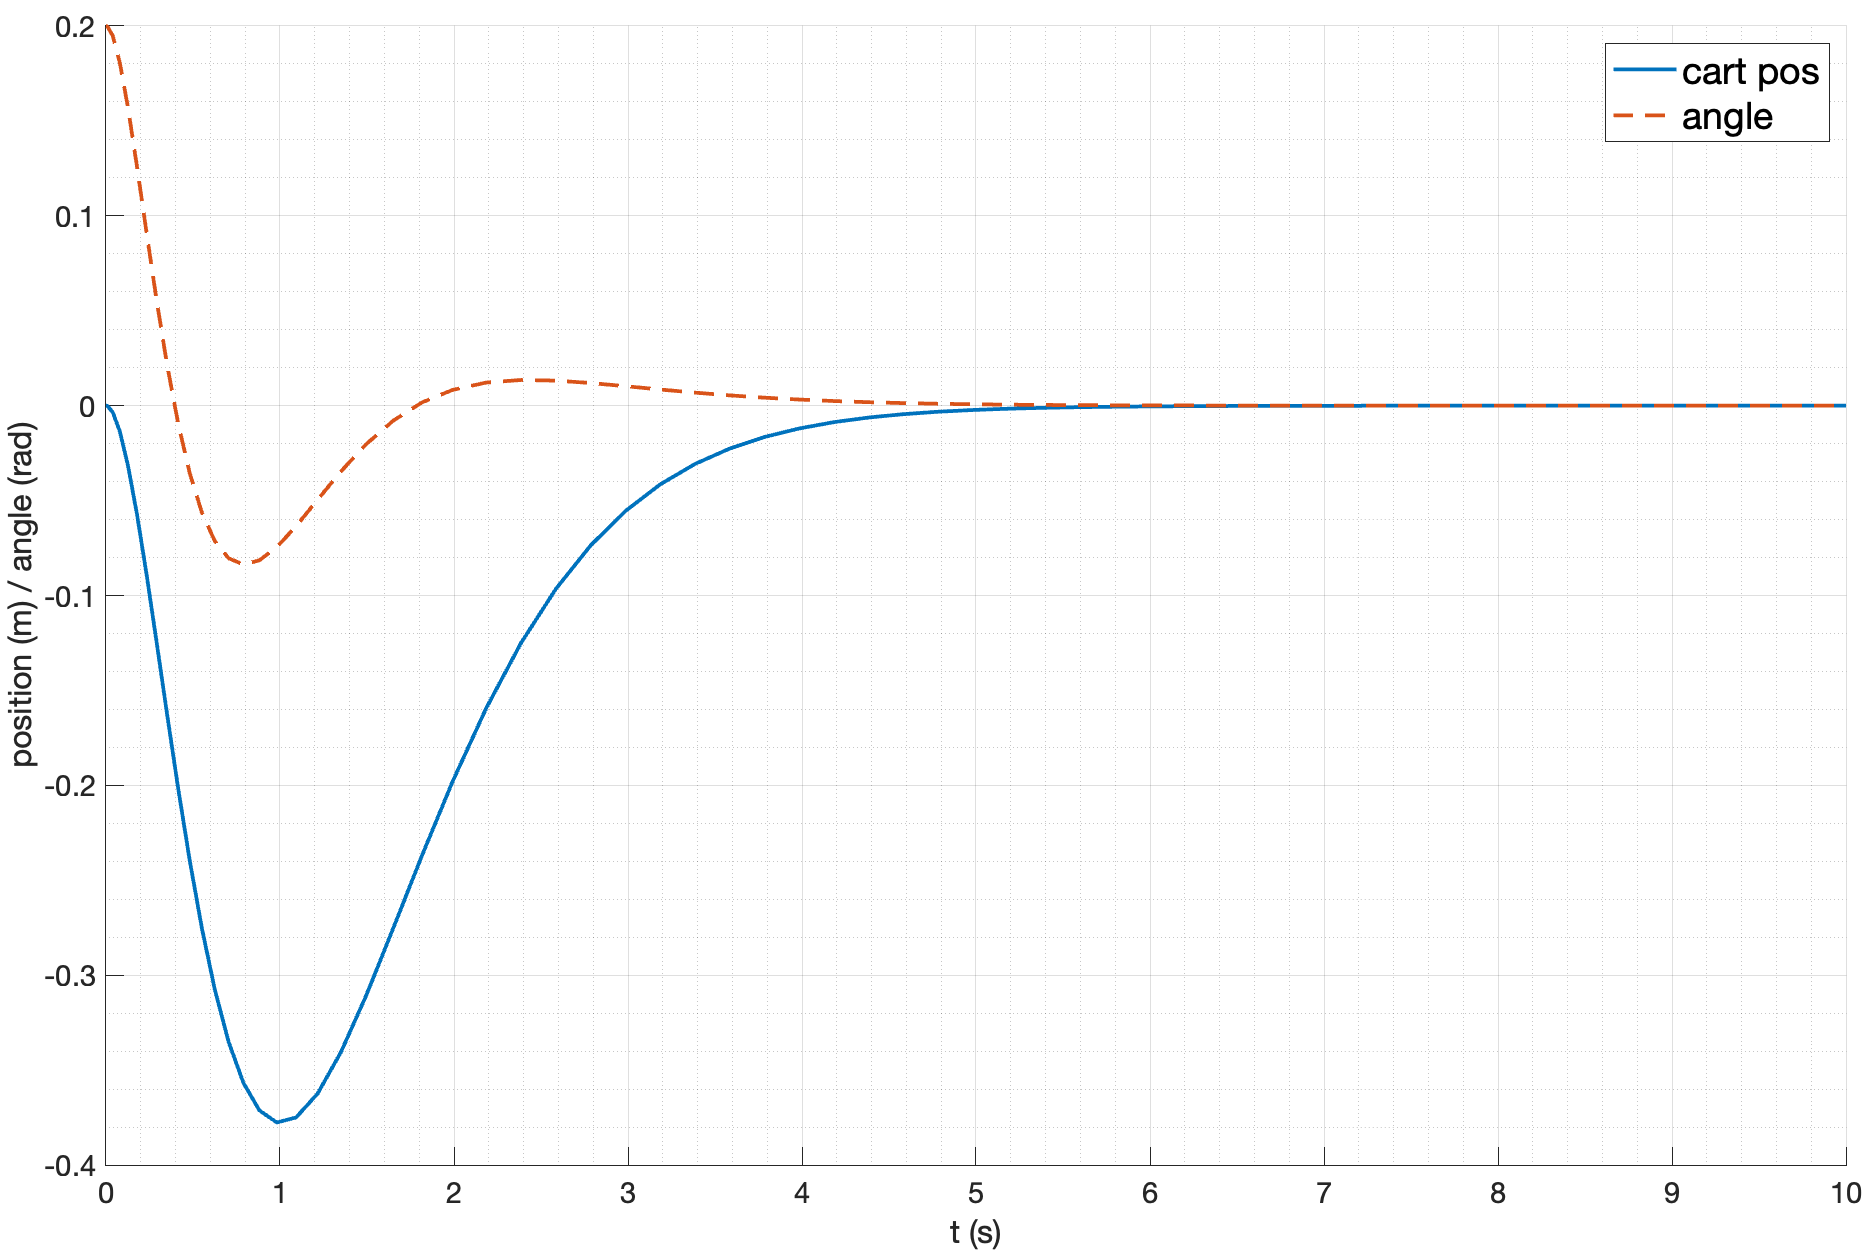
\includegraphics[width=\textwidth]{media/plots/modal_control/modal_control_linear_out.png}
    \caption{Результаты моделирования линейной модели системы с модальным регулятором}
    \label{fig:modal_control_linear_out}
\end{figure}

Можно заметить, что приходит в равновесное состояние. Теперь попробуем использовать этот же 
модальный регулятор на нелинейной модели системы. Схема моделирования приведена на
рисунке \ref{fig:modal_control_scheme_nonlinear}. Результаты моделирования приведены на
рисунке \ref{fig:modal_control_nonlinear_out}.


